%!TEX root = project.tex

\chapter*{About this project}
 % A brief description of what the project is, in about two-hundred and fifty words.
 
 
 
 Welcome to my minor Dissertation my name is Tomás O'Malley (G00361128) and I am a final year student studying  a Bsc Honours in Software Development @ Galway Mayo Institute of Technology. After my years of study and my deep interest in technology and how we interface device day-to-day I settled on developing a social network for local communities.What is a social network ?\\ \\ 
 
 A network of social interactions and personal relationships , common examples of social media platform include Facebook , Instagram and twitter. Smartphones have become an addition to how humans socialize and congregate, my applications target audience are people who want to congregate in local communities and share their photos , experiences and safely create events in their chosen communities with ease using their smart device. \\
 
 Each component from the back-end written in the secure language  of ruby on rails to the database system mongodb.This document outlines in great detail the many system design/architecture.Tackling a modern architecture will challenge and award when in an industrial environment.\\
 
 The application is focused around users such as rookies and administrators.User can use the forums to upload documents , private message each other and use  built in schedules to manage a healthy online and offline social life.\\
 
 This application incorporates some of the juggernauts  areas of modern day computing such as databases , web frameworks and mobile devices.All of the programming will be stored and document using the version control Git at \href{https://github.com/OmalleyTomas98/MinorDissertation}{Github} \\
 
 


\paragraph{Author}
 % Explain here who the authors are.
  The whole project was developed by Tomás O'Malley (G00361128) all project work and material can be found using my \href{https://github.com/OmalleyTomas98/MinorDissertation}{GitHub} \\The project was developed using an agile methodology to make sure I deliver a crucial component on time.
 You can find more about me via my Online College Portfolio  \href{https://omalleytomas98.github.io}{Here}


\chapter{Introduction}


 \subsection{ Project Aims}
 
 
 
 
 
 \subsection{ Project Metrics}
  \subsection{ Chapters analyzed }
    \subsection{ Project  Specification }
    
    
Here are a list of the features that will be Incorporated into the application to 
    \begin{itemize}
  \item User must  be able to log in and log out.
  \item Must be able to edit account details.
  \item Log in must be persistent throughout a session
  \item User Must be able to register an account.
  \item User Must be able to upload and edit profile follow.
  \item User can upload a post to forum.
  \item User can comment on posts on forum .
  \item Users credentials must be stored safely and encrypted on the database System
\end{itemize}
    
    
    
    \subsection{ Project  Context }



 % The introduction should be about three to five pages long.
% Make sure you use references~\cite{einstein}

Hello my name is Tomás O'Malley and I am a fourth year Galway student studying Software Development.It is mandatory for completion of our Bsc Honours in Software to deliver a Final Year Project and Dissertation  to ensure we have a tight grasp on computing before continuing our studies or working in a professional environment.\\

\\During our College Introduction during week 1 Semester 7 I decided to begin brainstorming for both modern technologies and the implications of these technologies in modern day.The Project needed to be delivered/developed starting from week 1 and completed by the end of semester 2.\\

It was crucial to begin planning once I was delegated a project supervisor (Dr John French) for the module "Applied Project and Minor Dissertation".



\chapter{Methodology}
    \subsection{ Version Control  }
    Version control is a system that records changes to a file or set of files over time so that you can recall specific versions later. ... Using a VCS also generally means that if you screw things up or lose files, you can easily recover.The version tool I will be using for development is named 'Github'

What is GitHub ? GitHub, Inc. is an American multinational corporation that provides hosting for software development and version control using Git. It offers the distributed version control and source code management functionality of Git, plus its own features. 
    

    \begin{center}    
      
\includegraphics[width=0.8\textwidth]{final-year-project-template-master/img/githubBanner.jpeg}
      \caption{GitHub}
  \label{fig:github1}

      
      


    \end{center}
    
    
    \subsection{ Development methodologies }
    
    
In software development, agile practices approach discovering requirements and developing solutions through the collaborative effort of self-organizing and cross-functional teams and their customer/end user    
    
    
    

    \begin{center}    
      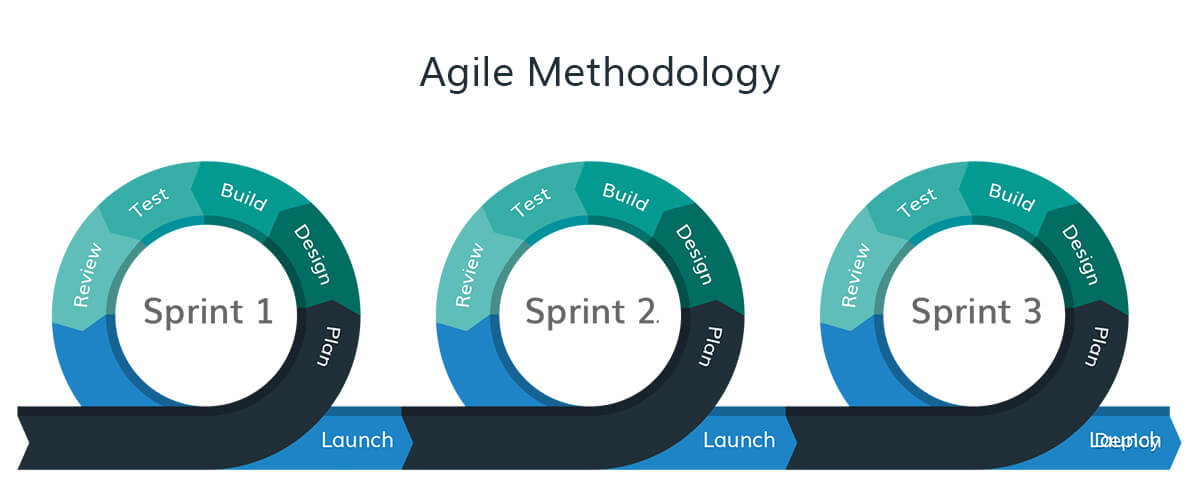
\includegraphics[width=0.8\textwidth]{final-year-project-template-master/img/agileSprint.jpg}
      
      
      


    \end{center}
    \subsection{ Development Environment  }
    \subsection{ Setting Objectives   }
    \subsection{ Testing approach   }




\begin{itemize}
\item %  Provide a context for your project.
The aim for my 2020/2021 FYP is to develop a mobile  Social Media Platform for local communities.
\item % Set out the objectives of the project
Objectives of project. (1) Create a social media application that can be used on mobile devices.(2) Research and learn the Ruby on rails language. (3) Learn the security protocols and incorporate  a strong back-end to safely store medias.(3) Create a secure and well defined database system using mongodb database systems. (4) Develop a clear understanding of User e
\item Briefly list each chapter / section and provide a 1-2 line description of what each section contains.
\item List the resource URL (GitHub address) for the project and provide a brief list of the main elements at the URL.
\end{itemize}



\chapter{Technology Review}




\subsection{Database System MongoDB}

What is MongoDB ?MongoDB is a cross-platform document-oriented database program. Classified as a NoSQL database program, MongoDB uses JSON-like documents with optional schemas. 



\subsection{Front-End React }

 The front-end of the application refers to  The layer above the back end is the front end and it includes all software or hardware that is part of a user interface. Human or digital users interact directly with various aspects of the front end of a program


\subsection{Back-End Ruby } 
The Back-end of the application  refers to the  back end refers to parts of a computer application or a program's code that allow it to operate and that cannot be accessed by a user. 



What is Ruby ?Ruby is an interpreted, high-level, general-purpose programming language. It was designed and developed in the mid-1990s by Yukihiro "Matz" Matsumoto in Japan.
\subsection{React Framework}



About one to two pages.
Describe the way you went about your project:
\begin{itemize}
\item  % Agile / incremental and iterative approach to development. Planning, meetings.
To make sure elements of the project were developed on time and at a level of quality I decided to use GitHub version control to manage my code base while adapting an agile approach by delegating tasks to myself and developing each component in a set time.Each week I arranged a time  with my project supervisor @ 10am Friday mornings where I delivered a LaTeX write up disclosing the many additions and obstacles of the project.


\item %  What about validation and testing? Junit or some other framework.

Automated testing will be in place to test the accuracy and responsiveness.


\item % If team based, did you use GitHub during the development process.

The whole project was developed by myself and Git Version control was incorporated into the project to make sure I timed the sprints 


\item % Selection criteria for algorithms, languages, platforms and technolo-gies.



\begin{enumerate}
  \item algorithms : Sorting algorithms bubble sort
  \item languages  : Ruby on rails , JavaScript , React Framework , noSQL.  
\item platforms  : Android Platform

\item Technologies   : Modern Social Media 

\end{enumerate}

\end{itemize}

\chapter{System Design}

\subsection{Application Overview  }
\subsection{Data  Management  }
\subsection{Logic   Management  }
\subsection{Application   Management }


 About seven to ten pages.
 
 
 
 log in system architecture 
 
 
 
 
 
\begin{itemize}
\item Describe each of the technologies you used at a conceptual level. Standards, Database Model (e.g. MongoDB, CouchDB), XMl, WSDL, JSON, JAXP.
\item Use references (IEEE format, e.g. [1]), Books, Papers, URLs (timestamp) – sources should be authoritative. 
\end{itemize}


\chapter{System Evaluation}
% As many pages as needed.

\subsection{Testing}
\subsection{Client Evaluation}
\subsection{Server Evaluation}
\subsection{Performance}
\subsection{Overall  Evaluation}





\begin{itemize}
\item Architecture, UML etc. An overview of the different components of the system. Diagrams etc… Screen shots etc.




\item Log In Procedure for new user base.Underneath is the flow chart of the program once the user enrolls or tries to enroll into the system.


{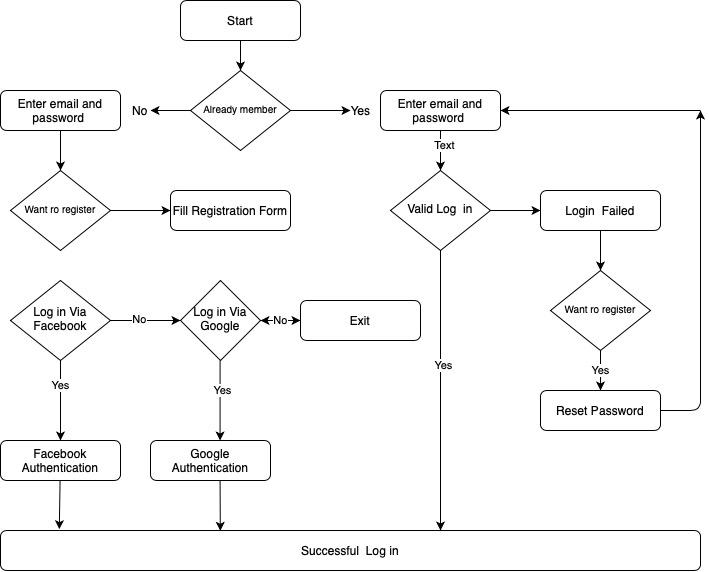
\includegraphics[width=1.0\textwidth]{final-year-project-template-master/img/Flowchart.jpg}}



\item Database Systems in place.For the product I have decided to incorporate the no-SQL approach using mongoDB to provide strong security and scaling for my program.

\href{https://medium.com/@rsk.saikrishna/when-to-use-mongodb-rather-than-mysql-d03ceff2e922}{MongoDB} 

\end{itemize}


\chapter{Conclusion}

\subsection{Overview}
\subsection{Project Outcome}
\subsection{Discoveries}
\subsection{Reflection}


 % As many pages as needed.
\begin{itemize}
\item  % Prove that your software is robust. How? Testing etc. 


Proof that the Project is robust is the use of the Database system NoSQL allows for large volumns of useres by adding new servers and shards in the database. The horizontal scaling process will be very easy. 

\href{https://stackoverflow.com/questions/4386949/is-nosql-is-suitable-for-social-networking-kind-of-applications}{Reference}


\item Use performance benchmarks (space and time) if algorithmic.
\item Measure the outcomes / outputs of your system / software against the objectives from the Introduction.
\item Highlight any limitations or opportuni-ties in your approach or technologies used.
\end{itemize}

\chapter{References and Appendices}
About three pages.






\begin{itemize}
\item Briefly summarise your context and ob-jectives (a few lines).
\item Highlight your findings from the evalua-tion section / chapter and any opportuni-ties identified.
\end{itemize}



